\subsection{QR Factorization}

\definition{QR Factorization} is a method to \textbf{decompose a matrix into two simpler matrices}: an \emph{orthogonal} matrix $Q$ and an \emph{upper triangular} matrix $R$.

\begin{flushleft}
    \textcolor{Red2}{\faIcon{exclamation-triangle} \textbf{Required prerequisites}}
\end{flushleft}
\begin{itemize}
    \item The \textbf{rank of a matrix is the maximum number of linearly independent rows or columns} in the matrix. Essentially, it tells us the dimension of the vector space spanned by the rows or columns. When we do Gaussian elimination, the number of non-zero rows represents the rank!
    
    \item An \textbf{orthogonal matrix} is a square matrix $Q$ with the property that its transpose is also its inverse. This means that $Q^{T} Q = Q Q^{T} = I$, where $I$ is the identity matrix. In simpler terms, the rows and columns of an orthogonal matrix are orthonormal vectors, each row and column is orthogonal to the others, and each has a length of 1 (norm equal to one).
    
    \item A \textbf{vector is orthogonal to another vector if their dot product is zero}. If this is true, we say that the orthogonal vectors are \emph{\textbf{perpendicular} to each other}.

    \item An \textbf{orthonormal vector} is a vector that is both orthogonal to other vectors in a set and normalized (meaning it has a unit length of 1, norm equal to one). In a collection of orthonormal vectors, each vector is perpendicular to the others, and each has a length of one.

    \item The \textbf{span of a set of orthonormal vectors} is the set of all possible linear combinations of those vectors. If we have a set of orthonormal vectors $\left\{v_{1}, v_{2}, \dots, v_{k}\right\}$, their span is \textbf{every vector that can be written as}:
    \begin{equation*}
        c_{1}v_{1} + c_{2}v_{2} + \cdots + c_{k}v_{k}
    \end{equation*}
    Where $c_{1}, c_{2}, \dots, c_{k}$ are scalar coefficients.
\end{itemize}

\begin{flushleft}
    \textcolor{Green3}{\faIcon{square-root-alt} \textbf{Mathematical point of view}}
\end{flushleft}
Find orthonormal vectors $\left[\mathbf{q}_{1}, \mathbf{q}_{2}, \dots, \mathbf{q}_{n}\right]$ that span the successive spaces\break spanned by the columns of $A = \left[\mathbf{a}_{1}, \mathbf{a}_{2}, \dots, \mathbf{a}_{n}\right]$:
\begin{equation*}
    <\mathbf{a}_{1}> \: \subseteq \: <\mathbf{a}_{1}, \mathbf{a}_{2}> \dots \: \subseteq \: <\mathbf{a}_{1}, \mathbf{a}_{2}, \dots, \mathbf{a}_{n}>
\end{equation*}
This means that (for full rank $A$):
\begin{equation*}
    <\mathbf{a}_{1}, \mathbf{a}_{2}, \dots, \mathbf{a}_{j}> \: = \: <\mathbf{q}_{1}, \mathbf{q}_{2}, \dots, \mathbf{q}_{j}> \hspace{2em} \forall j = 1, \dots, n
\end{equation*}
A matrix of the previous form will appear:
\begin{equation*}
    \left[\mathbf{a}_{1} \: | \: \mathbf{a}_{2} \: | \: \cdots \: | \: \mathbf{a}_{n}\right]
    =
    \left[\mathbf{q}_{1} \: | \: \mathbf{q}_{2} \: | \: \cdots \: | \: \mathbf{q}_{n}\right]
    \cdot
    \begin{bmatrix}
        r_{11} & r_{12} & \cdots & r_{1n} \\
        0 & r_{22} & \cdots & \vdots \\
        0 & 0 & \ddots & r_{nn}
    \end{bmatrix}
\end{equation*}
That is:
\begin{equation*}
    A = \widehat{Q}\widehat{R}
\end{equation*}
This is called the \textbf{reduced QR factorization}.

\highspace
Let $A$ be an $m \times n$ matrix. The \textbf{full QR factorization} of $A$ is the factorization $A = QR$, where:
\begin{itemize}
    \item $Q$ is $m \times m$ orthogonal $Q Q^{T} = I$
    \item $R$ is $m \times n$ upper-trapezoidal
\end{itemize}
\begin{figure}[!htp]
    \centering
    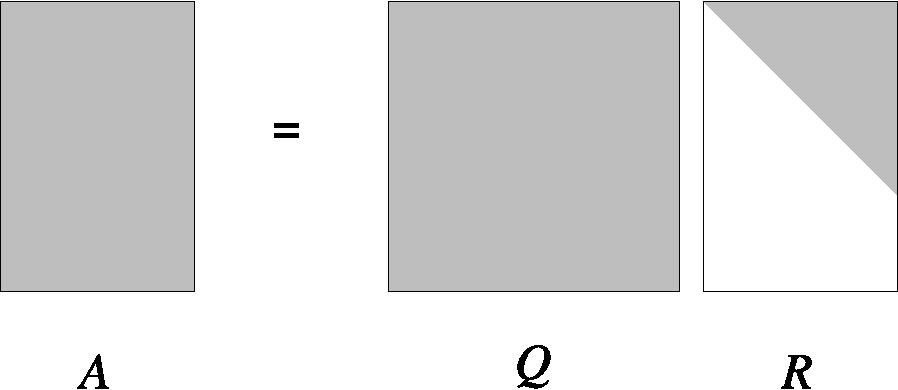
\includegraphics[width=.5\textwidth]{img/full-qr-factorization-1.pdf}
    \caption{Full QR Factorization.}
\end{figure}

\highspace
Let $A$ be an $m \times n$ matrix. The \textbf{reduced QR factorization} of $A$ is the factorization $A = \widehat{Q}\widehat{R}$, where:
\begin{itemize}
    \item $\widehat{Q}$ is $m \times m$
    \item $\widehat{R}$ is $m \times n$ upper-trapezoidal
\end{itemize}
\begin{figure}[!htp]
    \centering
    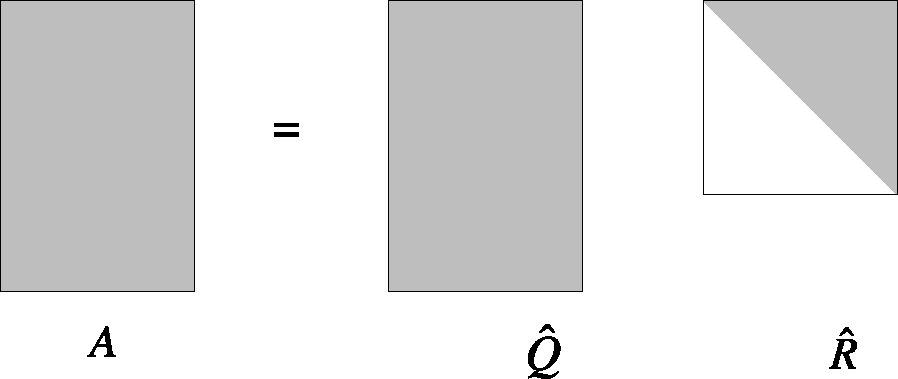
\includegraphics[width=.5\textwidth]{img/reduced-qr-factorization-1.pdf}
    \caption{Reduced QR Factorization.}
\end{figure}

\noindent
Every matrix $A \in \mathbb{C}^{m \times n}$ ($m \ge n$) has a \textbf{full QR factorization and a reduced QR factorization}. Also, every $A$ of \textbf{full rank has a unique reduced QR factorization} with $r_{jj} > 0$, $j = 1, \dots, n$.

\newpage

\begin{flushleft}
    \textcolor{Green3}{\faIcon{question-circle} \textbf{What is Gram-Schmidt orthogonalization and why is it important?}}
\end{flushleft}
After a long mathematical introduction to the full and reduced QR factorization methods, the question is \emph{how can we apply this in practice}? Well, finding a special set of vectors that satisfies some properties cannot be very easy. Fortunately, \definition{Gram-Schmidt orthogonalization} is one of the primary \textbf{methods used to find the orthogonal (or orthonormal) vectors} necessary for QR factorization.

\highspace
The Gram-Schmidt orthogonalization takes as:
\begin{itemize}
    \item \textbf{Input}. A set of vectors (typically the columns of the matrix $A$).
    
    \item \textbf{Output}. An orthogonal set of vectors, which can then be normalized to form an orthonormal set.
\end{itemize}

\highspace
Mathematically, the Gram-Schmidt orthogonalization works as follows. Given the columns of $A$ $\mathbf{a}_{1}, \mathbf{a}_{2}, \dots, \mathbf{a}_{n}$; find new $\mathbf{q}_{j}$ (the $j$-th column of $\widehat{Q}$) orthogonal to $\mathbf{q}_{1}, \dots, \mathbf{q}_{j-1}$ by subtracting components along previous vectors:
\begin{equation*}
    \mathbf{w}_{j} = \mathbf{a}_{j} - \displaystyle\sum_{k=1}^{j-1} \left(\overline{\mathbf{q}}_{k}^{T}\mathbf{a}_{j}\right)\mathbf{q}_{k}
\end{equation*}
Normalize to get $\mathbf{q}_{j} = \dfrac{\mathbf{w}_{j}}{\left|\left|\mathbf{w}_{j}\right|\right|}$, we then obtain a reduced QR factorization with:
\begin{equation}
    r_{ij} = \overline{\mathbf{q}}_{i}^{T}\mathbf{a}_{j} \hspace{2em} i \ne j
\end{equation}
And:
\begin{equation*}
    r_{jj} = \left|\left|\mathbf{a}_{j} - \displaystyle\sum_{i=1}^{j-1} r_{ij}\mathbf{q}_{i}\right|\right|
\end{equation*}
Since the previous equation $r_{ij}$ is numerically unstable because it is too sensitive to rounding errors, the following modification ensures more stability. The previous one is called \definition{Classical Gram-Schmidt (CGS, or simply GS)}, and the following one is called \definition{Classical Gram-Schmidt (CGS, or simply GS)}:
\begin{equation}
    r_{ij} = \overline{\mathbf{q}}_{i}^{T}\mathbf{w}_{j}
\end{equation}